\newpage

\section{Trigger}
\label{sec:trigger}


Events are selected if one of the following triggers has fired: HLT\_HT750, HLT\_PFHT650, HLT\_PFNoPUHT650
HLT\_FatDiPFJetMass750\_DR1p1\_Deta1p5.  All versions of each of these triggers is used. None of these triggers are prescaled druing the 2012 data taking period. HLT\_PFNoPUHT650 trigger is used for the data set after the RunC(including RunC), while HLT\_PFHT650
trigger is only used for RunA and RunB data sets. 


Figure ~\ref{fig:trigger efficiencies part1}, Figure ~\ref{fig:trigger efficiencies part2} and Figure ~\ref{fig:trigger efficiencies part3} shows the trigger efficiencies of the OR of the highest threshold HLT\_PFHT650 trigger and the HLT\_FatJetMass trigger w.r.t. an OR of the lower threshold HLT\_HT550 trigger. From the plot, the trigger is $99\%$ effiecient above $890 GeV$ for the untagged, single tagged and double tagged data. 


\begin{figure}[htb]
\centering
     \resizebox{0.75\linewidth}{!}{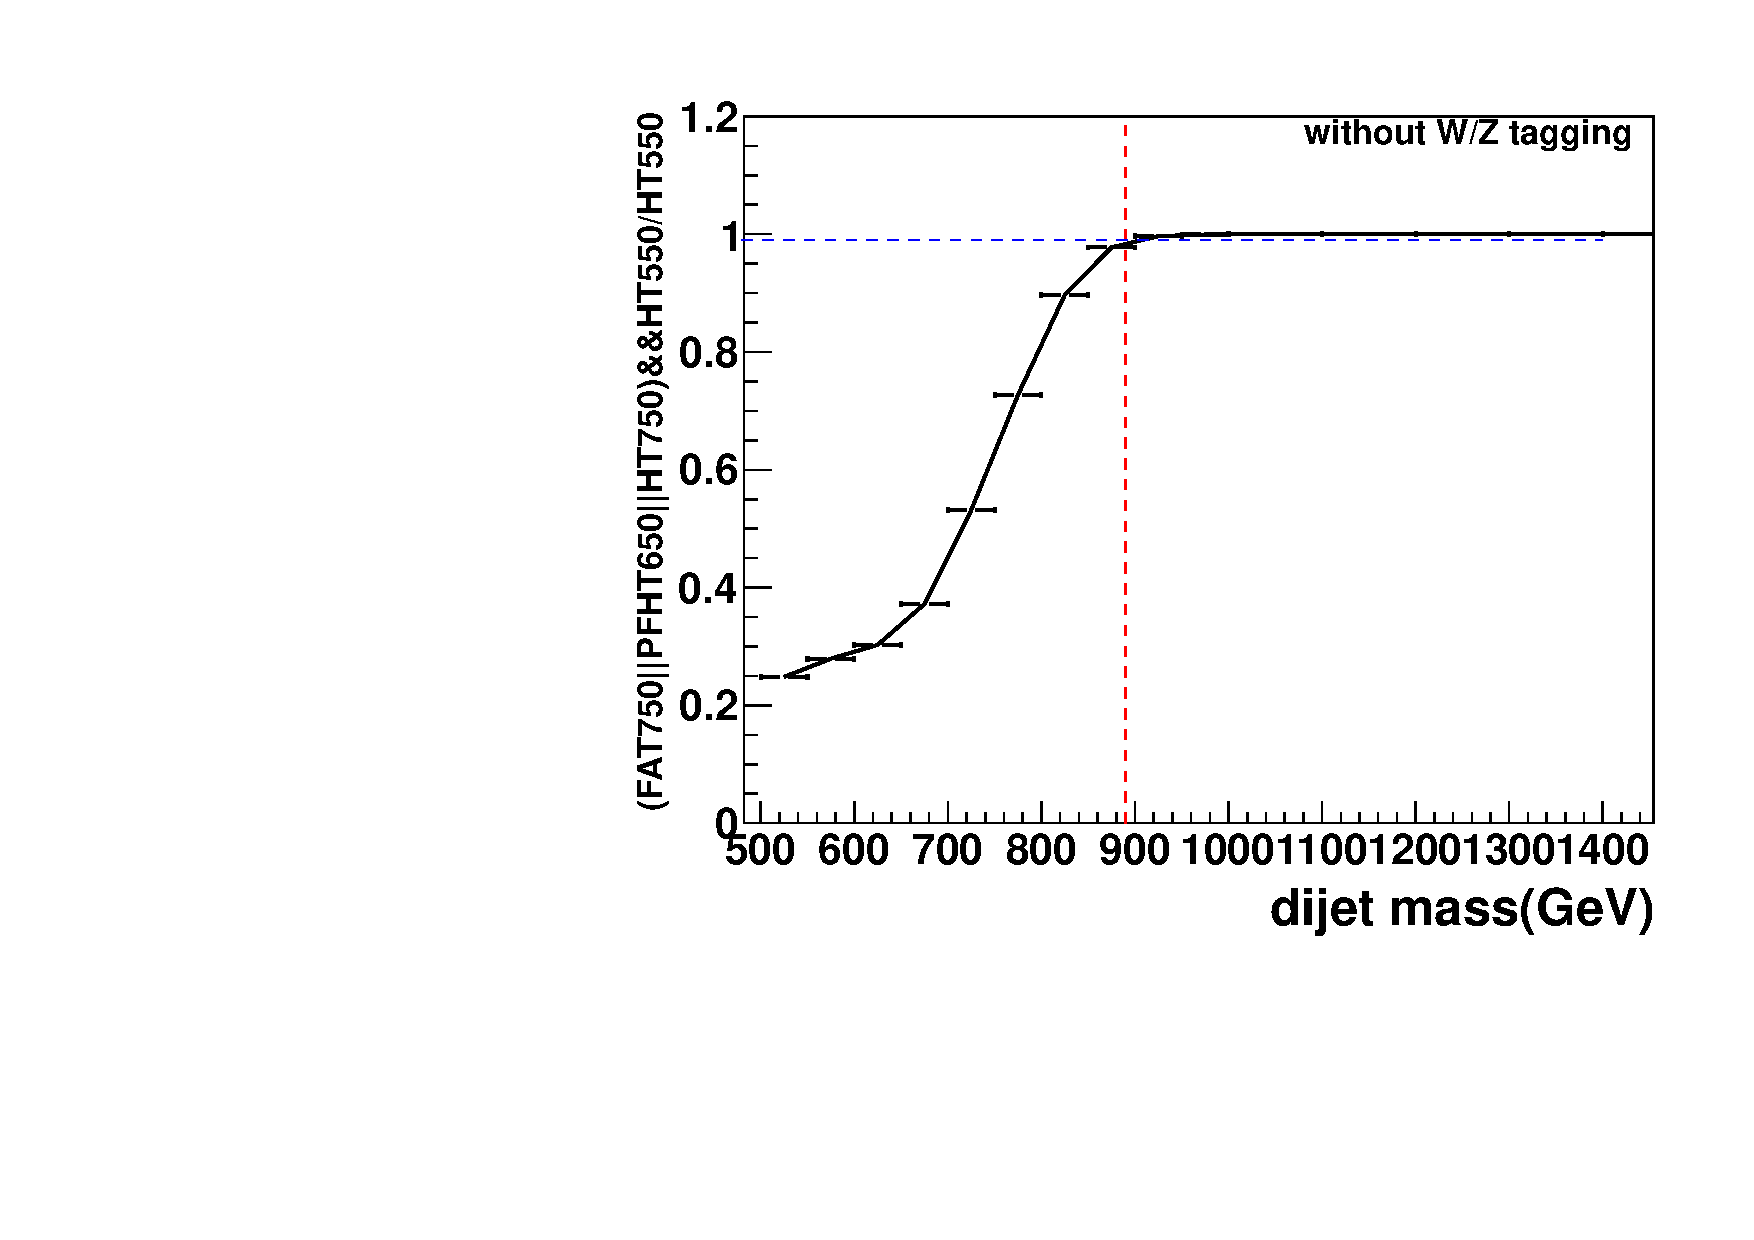
\includegraphics{figs/trigger-eff/Dataeff_withouttagging.pdf}} \\   
\caption[Trigger efficiencies]{Trigger efficiency for untagged data of FAT\_750$\parallel$HLT\_PF(NoPU)HT650$\parallel$HLT\_HT750 measured using data collected by lower threshold $H_T550$ trigger. The dash red line is positioned at $m_{jj}$ equal $890 GeV$, the blue line is at efficiency at 99$\%$. }
  \label{fig:trigger efficiencies part1}
\end{figure}

\begin{figure}[htb]
\centering
     \resizebox{0.75\linewidth}{!}{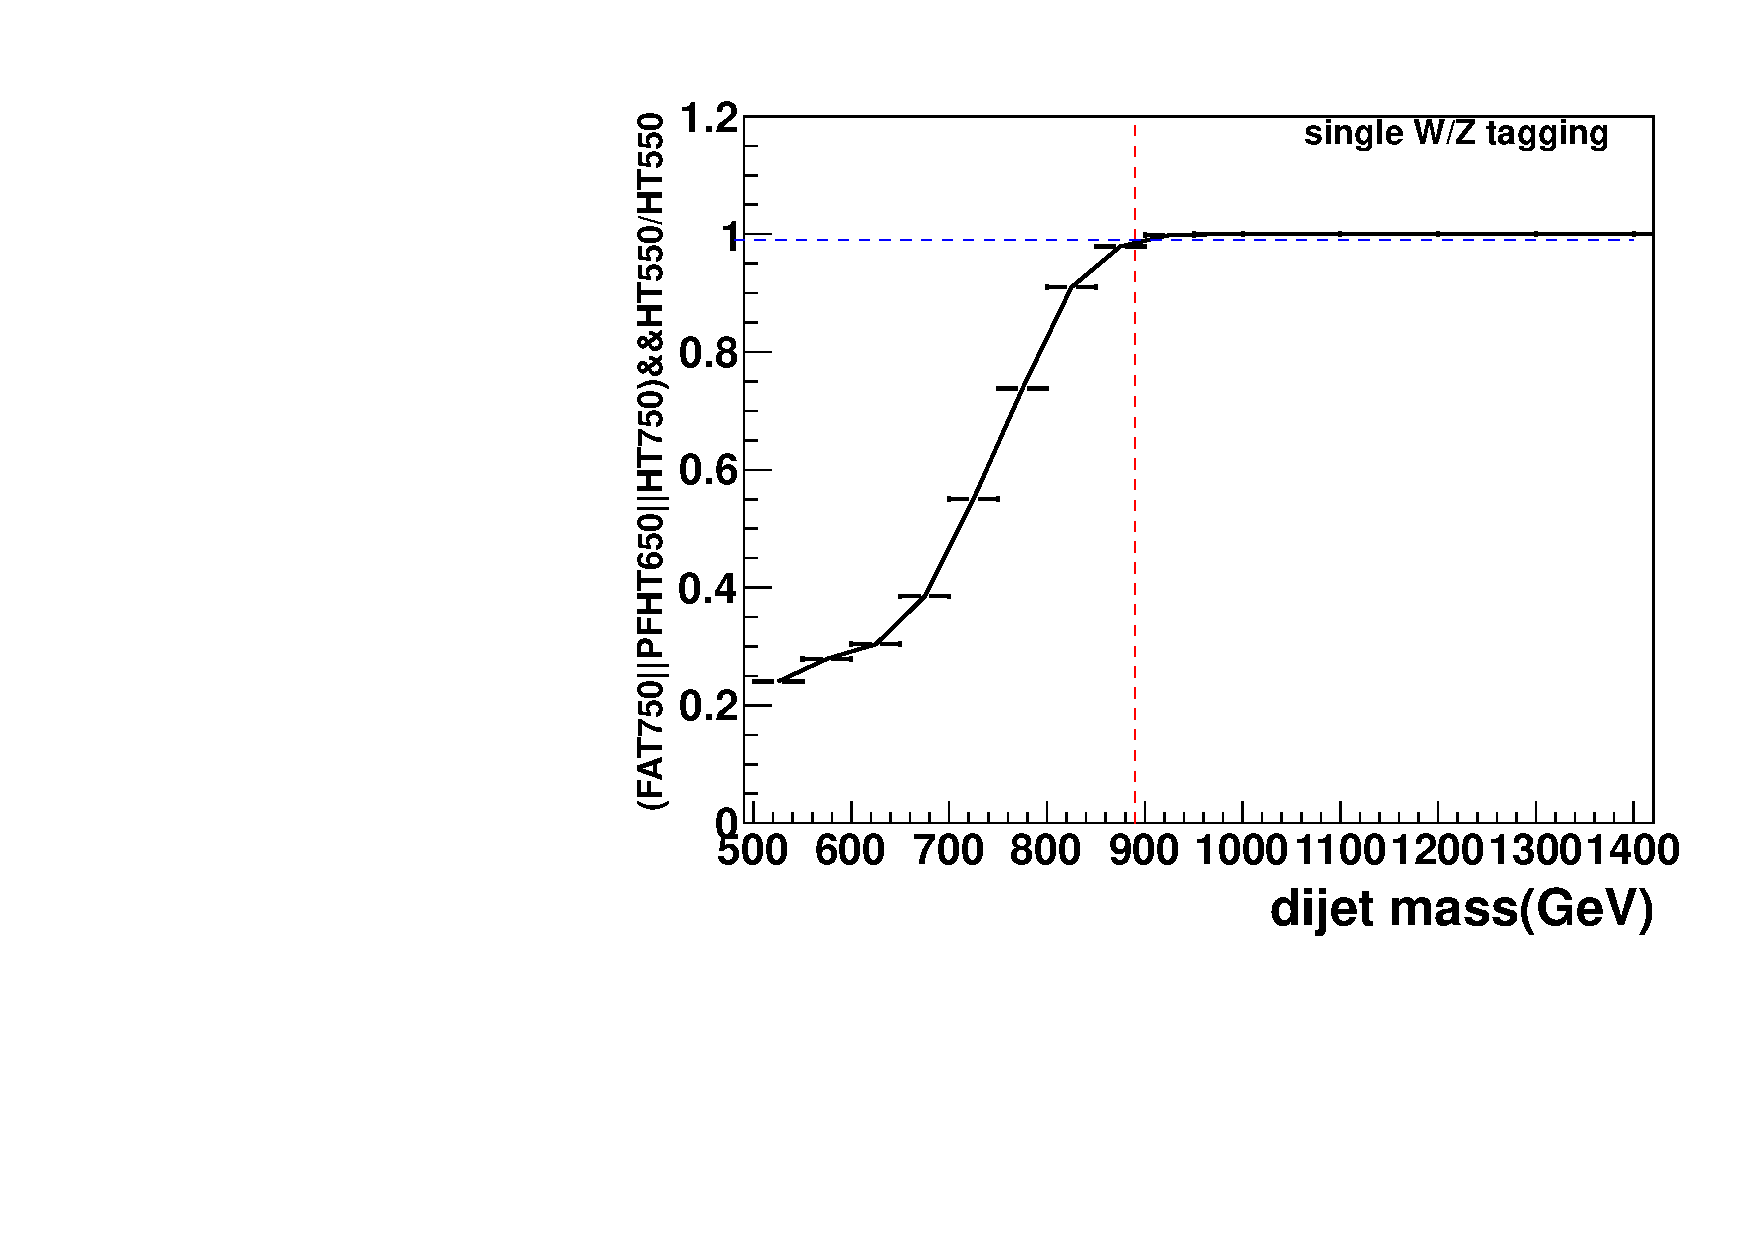
\includegraphics{figs/trigger-eff/Dataeff_singletagging.pdf}}  \\
\caption[Trigger efficiencies]{Trigger efficiency for single tagged data of FAT\_750$\parallel$HLT\_PF(NoPU)HT650$\parallel$HLT\_HT750 measured using data collected by lower threshold $H_T550$ trigger. The dash red line is positioned at $m_{jj}$ equal $890 GeV$, the blue line is at efficiency at 99$\%$. }
  \label{fig:trigger efficiencies part2}
\end{figure}

\begin{figure}[htb]
\centering
     \resizebox{0.75\linewidth}{!}{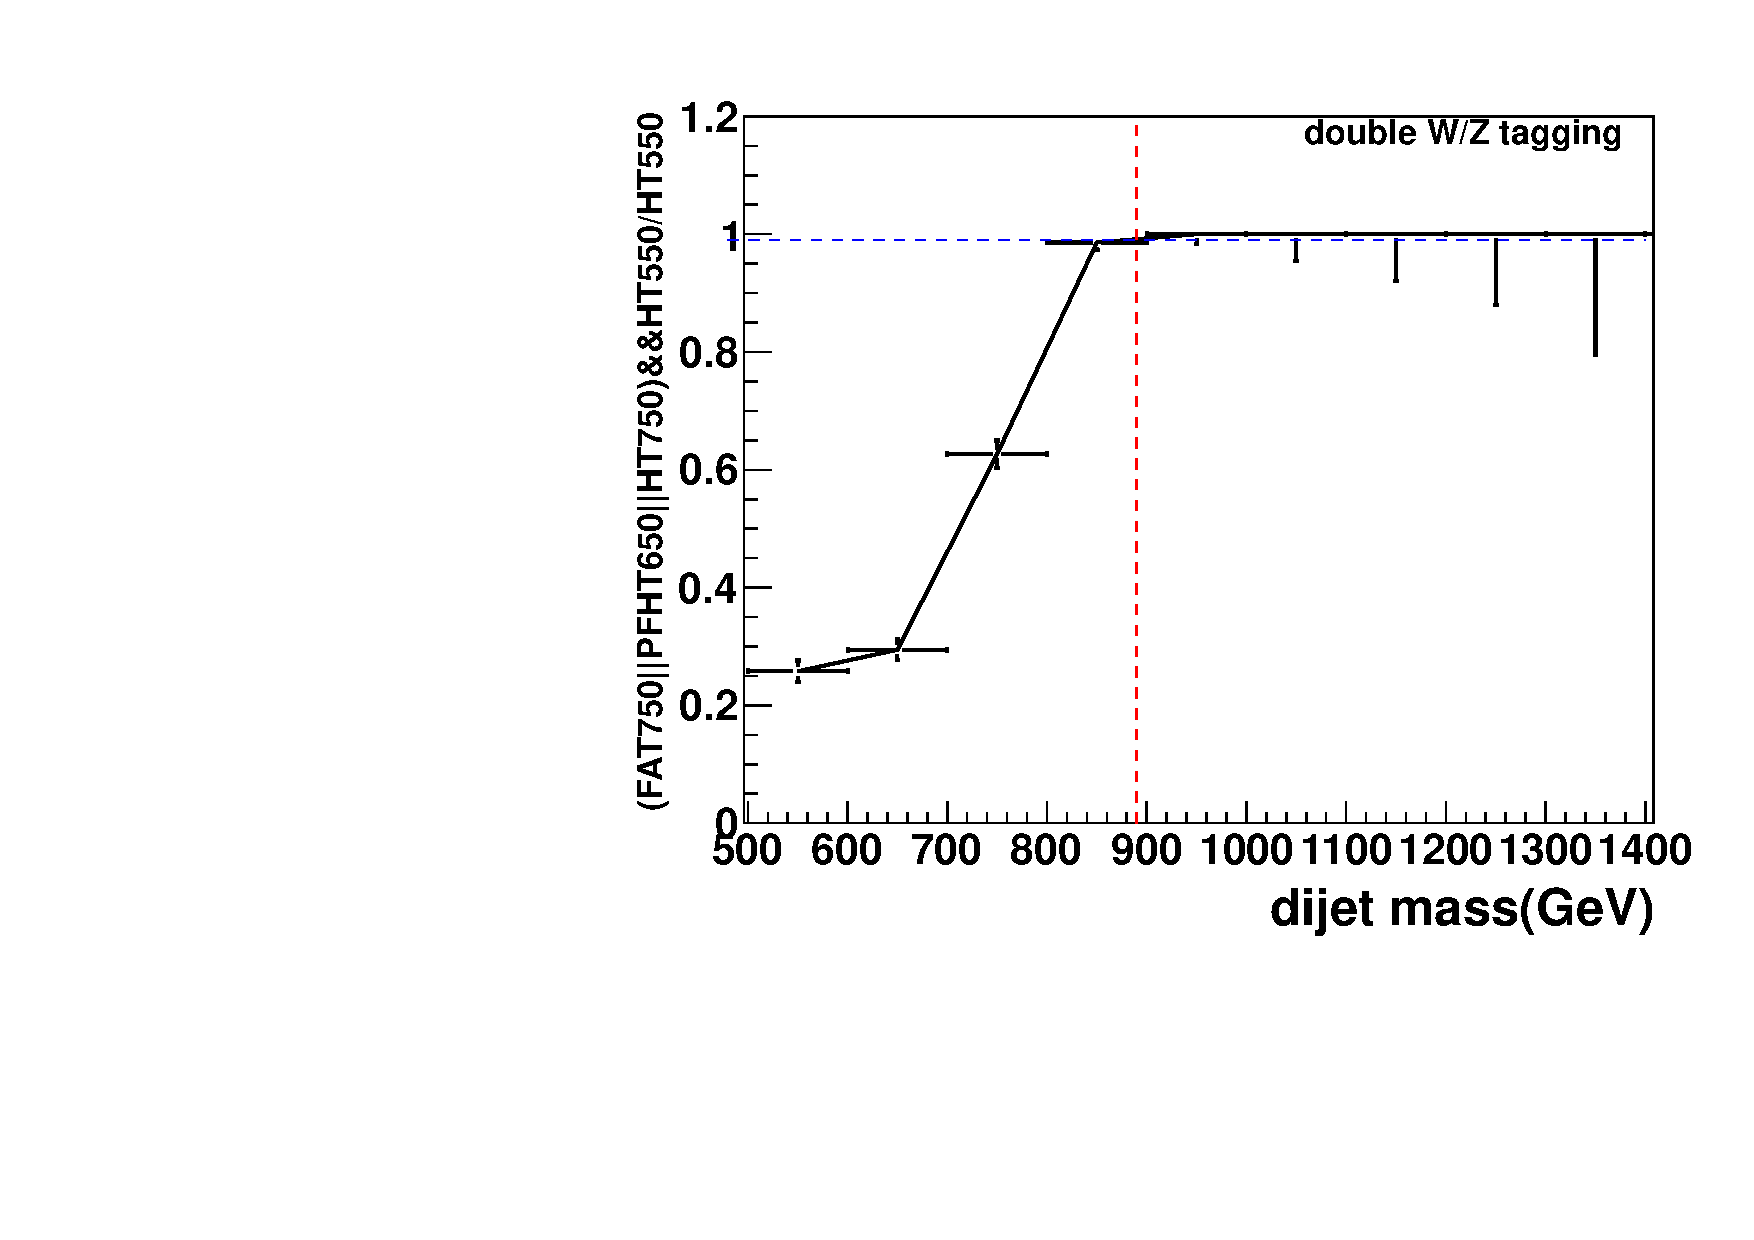
\includegraphics{figs/trigger-eff/Dataeff_doubletagging.pdf}} \\
\caption[Trigger efficiencies]{Trigger efficiency for double tagged data of FAT\_750$\parallel$HLT\_PF(NoPU)HT650$\parallel$HLT\_HT750 measured using data collected by lower threshold $H_T550$ trigger. The dash red line is positioned at $m_{jj}$ equal $890 GeV$, the blue line is at efficiency at 99$\%$. }
  \label{fig:trigger efficiencies part3}
\end{figure}


\clearpage













